%%%%%%%%%%%%%%%%%%%%%%%%%%%%%%%%%%%%%%%%%
% baposter Landscape Poster
% LaTeX Template
% Version 1.0 (11/06/13)
%
% baposter Class Created by:
% Brian Amberg (baposter@brian-amberg.de)
%
% This template has been downloaded from:
% http://www.LaTeXTemplates.com
%
% License:
% CC BY-NC-SA 3.0 (http://creativecommons.org/licenses/by-nc-sa/3.0/)
%
%%%%%%%%%%%%%%%%%%%%%%%%%%%%%%%%%%%%%%%%%

%----------------------------------------------------------------------------------------
%	PACKAGES AND OTHER DOCUMENT CONFIGURATIONS
%----------------------------------------------------------------------------------------

%\documentclass[landscape,a0paper,fontscale=0.285]{baposter} % Adjust the font scale/size here
\documentclass[landscape,a1paper,fontscale=0.450]{baposter} % Adjust the font scale/size here 

\usepackage{graphicx} % Required for including images
\graphicspath{{figures/}} % Directory in which figures are stored

\usepackage{amsmath} % For typesetting math
\usepackage{amssymb} % Adds new symbols to be used in math mode
\usepackage{units}

\usepackage{booktabs} % Top and bottom rules for tables
\usepackage{enumitem} % Used to reduce itemize/enumerate spacing
\usepackage{palatino} % Use the Palatino font
\usepackage[font=small,labelfont=bf]{caption} % Required for specifying captions to tables and figures
\usepackage{lipsum}

\usepackage{multicol} % Required for multiple columns
\setlength{\columnsep}{1.5em} % Slightly increase the space between columns
\setlength{\columnseprule}{0mm} % No horizontal rule between columns

\usepackage{tikz} % Required for flow chart
\usetikzlibrary{shapes,arrows} % Tikz libraries required for the flow chart in the template

\newcommand{\compresslist}{ % Define a command to reduce spacing within itemize/enumerate environments, this is used right after \begin{itemize} or \begin{enumerate}
\setlength{\itemsep}{1pt}
\setlength{\parskip}{0pt}
\setlength{\parsep}{0pt}
}

\definecolor{lightblue}{rgb}{0.145,0.6666,1} % Defines the color used for content box headers
\definecolor{maroon}{rgb}{0.5,0,0} % Defines the color used for content box headers
\newcommand{\vect}[1]{\boldsymbol{#1}}
\newcommand{\NN}{\mathcal N}
\DeclareMathOperator*{\argmin}{arg\,min}
\begin{document}

\begin{poster}
{
headerborder=closed, % Adds a border around the header of content boxes
colspacing=1em, % Column spacing
bgColorOne=white, % Background color for the gradient on the left side of the poster
bgColorTwo=white, % Background color for the gradient on the right side of the poster
borderColor=maroon, % Border color
headerColorOne=black, % Background color for the header in the content boxes (left side)
headerColorTwo=maroon, % Background color for the header in the content boxes (right side)
headerFontColor=white, % Text color for the header text in the content boxes
boxColorOne=white, % Background color of the content boxes
textborder=roundedleft, % Format of the border around content boxes, can be: none, bars, coils, triangles, rectangle, rounded, roundedsmall, roundedright or faded
eyecatcher=true, % Set to false for ignoring the left logo in the title and move the title left
headerheight=0.1\textheight, % Height of the header
headershape=roundedright, % Specify the rounded corner in the content box headers, can be: rectangle, small-rounded, roundedright, roundedleft or rounded
headerfont=\Large\bf\textsc, % Large, bold and sans serif font in the headers of content boxes
%textfont={\setlength{\parindent}{1.5em}}, % Uncomment for paragraph indentation
linewidth=2pt % Width of the border lines around content boxes
}
%----------------------------------------------------------------------------------------
%	TITLE SECTION 
%----------------------------------------------------------------------------------------
%
{} % First university/lab logo on the left
{\bf\textsc{Parametric entropy based density estimation in distance sampling}}%\vspace{0.5em}} % Poster title
{\textsc{\{ Kevin Joyce \} \hspace{12pt} The University of Montana}} % Author names and institution
{} % Second university/lab logo on the right

%----------------------------------------------------------------------------------------
%	Introduction
%----------------------------------------------------------------------------------------

\headerbox{Density estimation}{name=introduction,column=0,span=2,row=0}{

\begin{multicols}{2}
  
  \begin{center}
    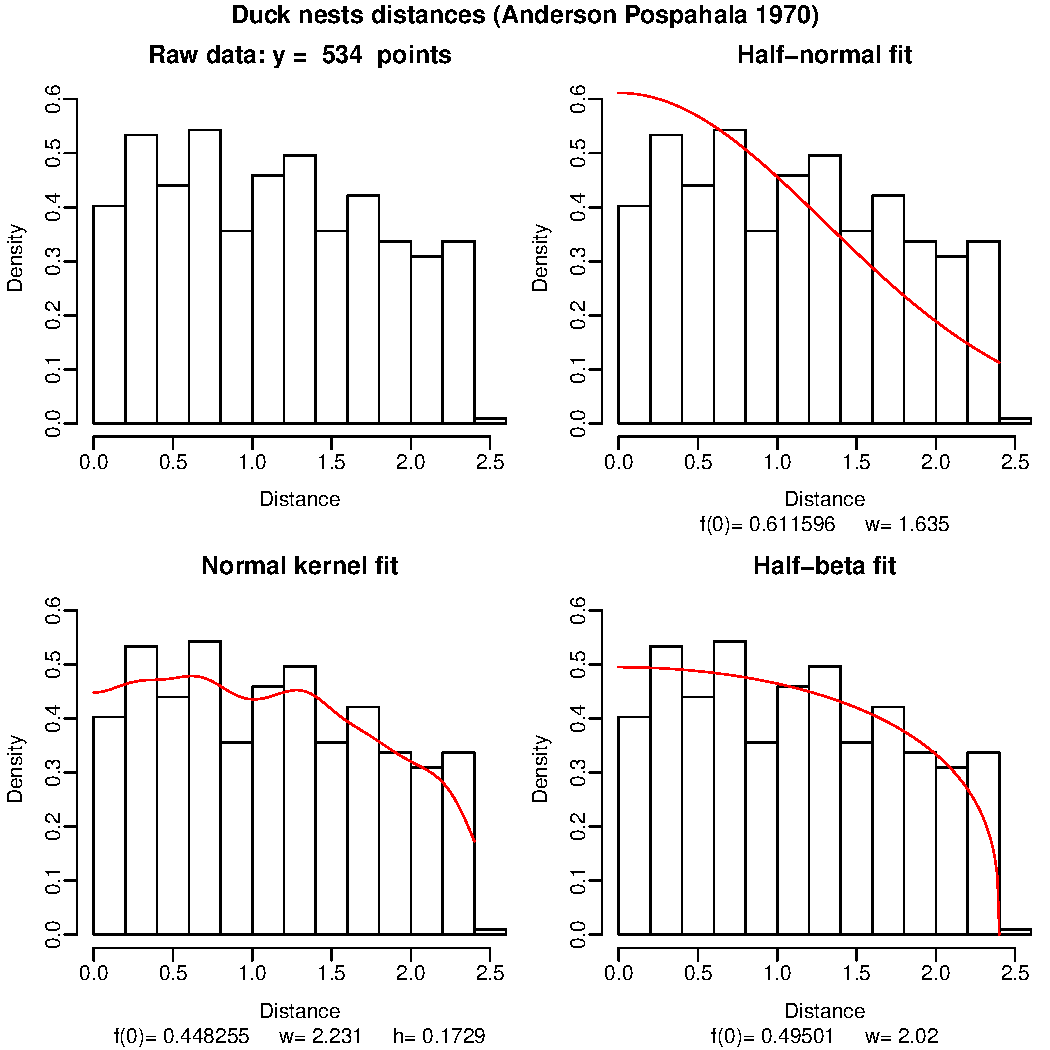
\includegraphics[width=.35\textwidth]{../duck_nest_fits.pdf}
  \end{center}
  \captionof{figure}{Distance data for duck nests in the Monte Vista National Wildlife Refuge in Colorado.}
  \vspace{1em}
  
  The problem of interest in this work is to estimate the density of objects in
  a known area from distance data collected along line-transects within the
  area.  This problem has been extensively studied, and much work involves
  estimation based on the density estimator
  \begin{equation}
    \hat D_i = \frac {y_i \hat f(0)}{2L_i}
  \end{equation}
  where $y_i$ are the enumerated counts along the $i$th transect, $L_i$ is the
  length of the $i$th transect\cite{buckland2001introduction}
   \cite{thompson2012sampling}. By far, the most involved part of the
  estimation is obtaining $\hat f(0)$, the peak of the probability distribution
  of the detected distances from the transect. This work is aimed at finding a robust
  parametric method for estimating $\hat f$ where detectability has relatively low kurtosis, or heavy central weighting within a fixed region.  \vspace{1cm}
\end{multicols}
}

%----------------------------------------------------------------------------------------
%	Estimating Entropy
%----------------------------------------------------------------------------------------

\headerbox{Estimating Entropy}{name=data,column=3,row=0,bottomaligned=introduction}{

%\begin{multicols}{2}
A well-known result from mathematical statistics states that if a random
variable $X$ is distributed with a cumulative distribution function (CDF)
$F(x)$, then the random variable $U=F(X)$ is distributed uniformly
over $[0,1]$. Of all random variables supported on $[0,1]$ with density
function $f(x)$, it can be shown that the entropy statistic 
\begin{equation}
  H(X) = \int_{0}^1 f \log f\,dx
\end{equation}
is maximized when the distribution is uniform
\cite{cover2006elements}. There is much work on estimating the entropy
statistic , and we employ a straight-forward histogram based estimator
\begin{equation}
  \widehat H = \sum_{\mathrm{bins}} f(n_i) \log \frac{f(n_i)}{w_i}.
\end{equation}
This is known to be MLE \cite{cover2006elements} and has been implemented in
\texttt R in the freely available \texttt{CRAN} library \texttt{entropy}. 
%\end{multicols}
%\vspace{0.3em} % When there are two boxes, some whitespace may need to be added if the one on the right has more content
}

%----------------------------------------------------------------------------------------
%	Beta Family Function
%----------------------------------------------------------------------------------------

\headerbox{Beta Distribution}{name=model,column=2,row=0,bottomaligned=data}{
Of distributions supported on the interval $[0,1]$, symmetric beta distributions form a flexible parametric family given by
\begin{equation}
  f(x) = B(\alpha) x^\alpha (1-x)^\alpha
\end{equation}
%This single parameter family can be optimized to fit density data as illustrated below.
\begin{center}
  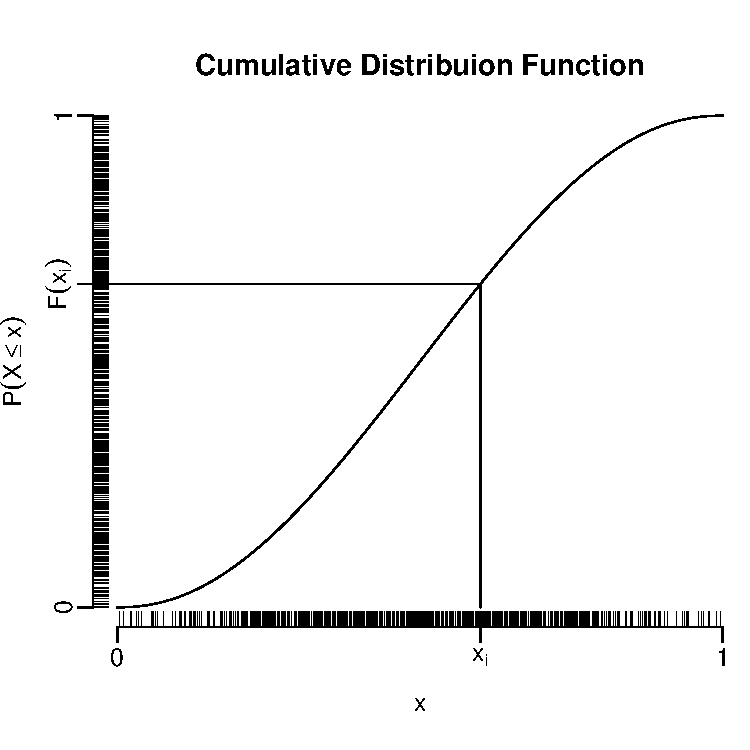
\includegraphics[width=.5\textwidth]{../cdf_example.pdf}
  \captionof{figure}{Finitely supported density data mapped through a beta CDF that maximizes entropy.}
\end{center}
}
%----------------------------------------------------------------------------------------
%	FUTURE RESEARCH
%----------------------------------------------------------------------------------------

\headerbox{Conclusions}{name=futureresearch,column=0,span=3,above=bottom}{ % This block is as tall as the references block

\begin{multicols}{3}
  The half-normal estimator appears to be bimodal with a large positive bias.  The normal kernel estimate is skewed
  right, but appears to be relatively unbiased in estimating the total.  Our
  estimator has a significantly lower variance than the normal kernel
  estimator, but appears to have a positive bias and slight biomodality.  In the figure to the right,
  it can be seen that the normal kernel estimator seems to overfit 
  densities which may be the for the larger variance in the population total estimator.  The
  EM half-beta estimator, on the other hand, appears to be more stable.  Note that
  it is constrained to have zero probability at the maximum data value, and this could
  be the reason for the upward bias.  A modification to the curves to account
  for this may remove the bias.

  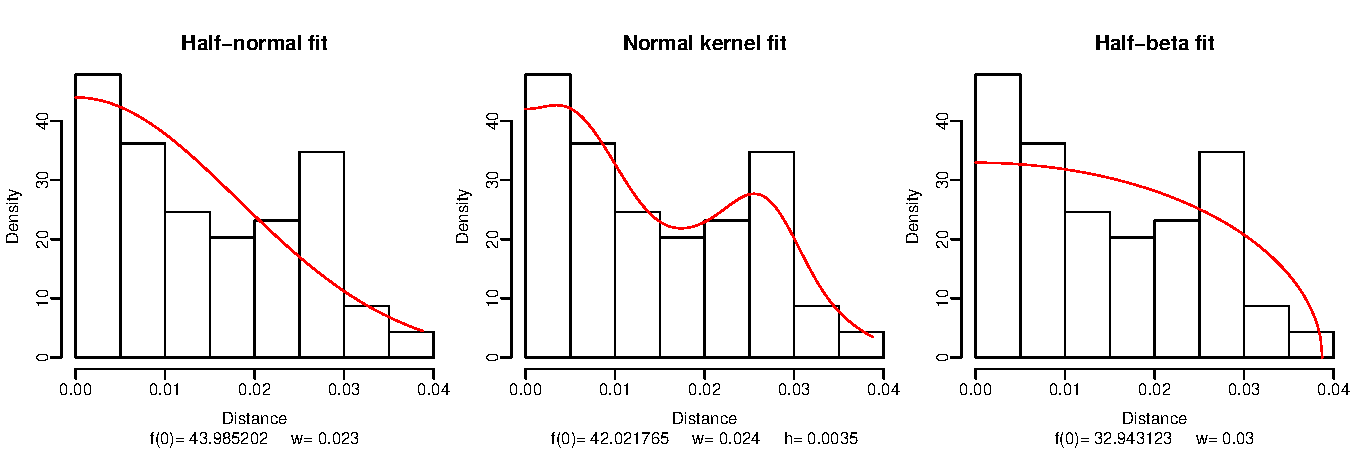
\includegraphics[width=.3\textwidth]{../problematic_kernel_fit.pdf}
  \vspace{1em}
\end{multicols}
}

%----------------------------------------------------------------------------------------
%	CONTACT INFORMATION
%----------------------------------------------------------------------------------------

%\headerbox{Future Work}{name=contact,column=2,aligned=futureresearch,above=bottom}{ % This block is as tall as the references block
%}

%----------------------------------------------------------------------------------------
%	REFERENCES
%----------------------------------------------------------------------------------------

\headerbox{References}{name=references,column=3,aligned=futureresearch,above=bottom}{

\renewcommand{\section}[2]{\vskip 0.05em} % Get rid of the default "References" section title
\nocite{*} % Insert publications even if they are not cited in the poster
\footnotesize{ % Reduce the font size in this block
\bibliographystyle{unsrt}
\bibliography{conference_poster_4} % Use sample.bib as the bibliography file
}}

%----------------------------------------------------------------------------------------
%     Simulation Results   
%----------------------------------------------------------------------------------------

\headerbox{Simulation Results}{name=results,column=2,span=2,row=0,below=model,above=futureresearch}{
  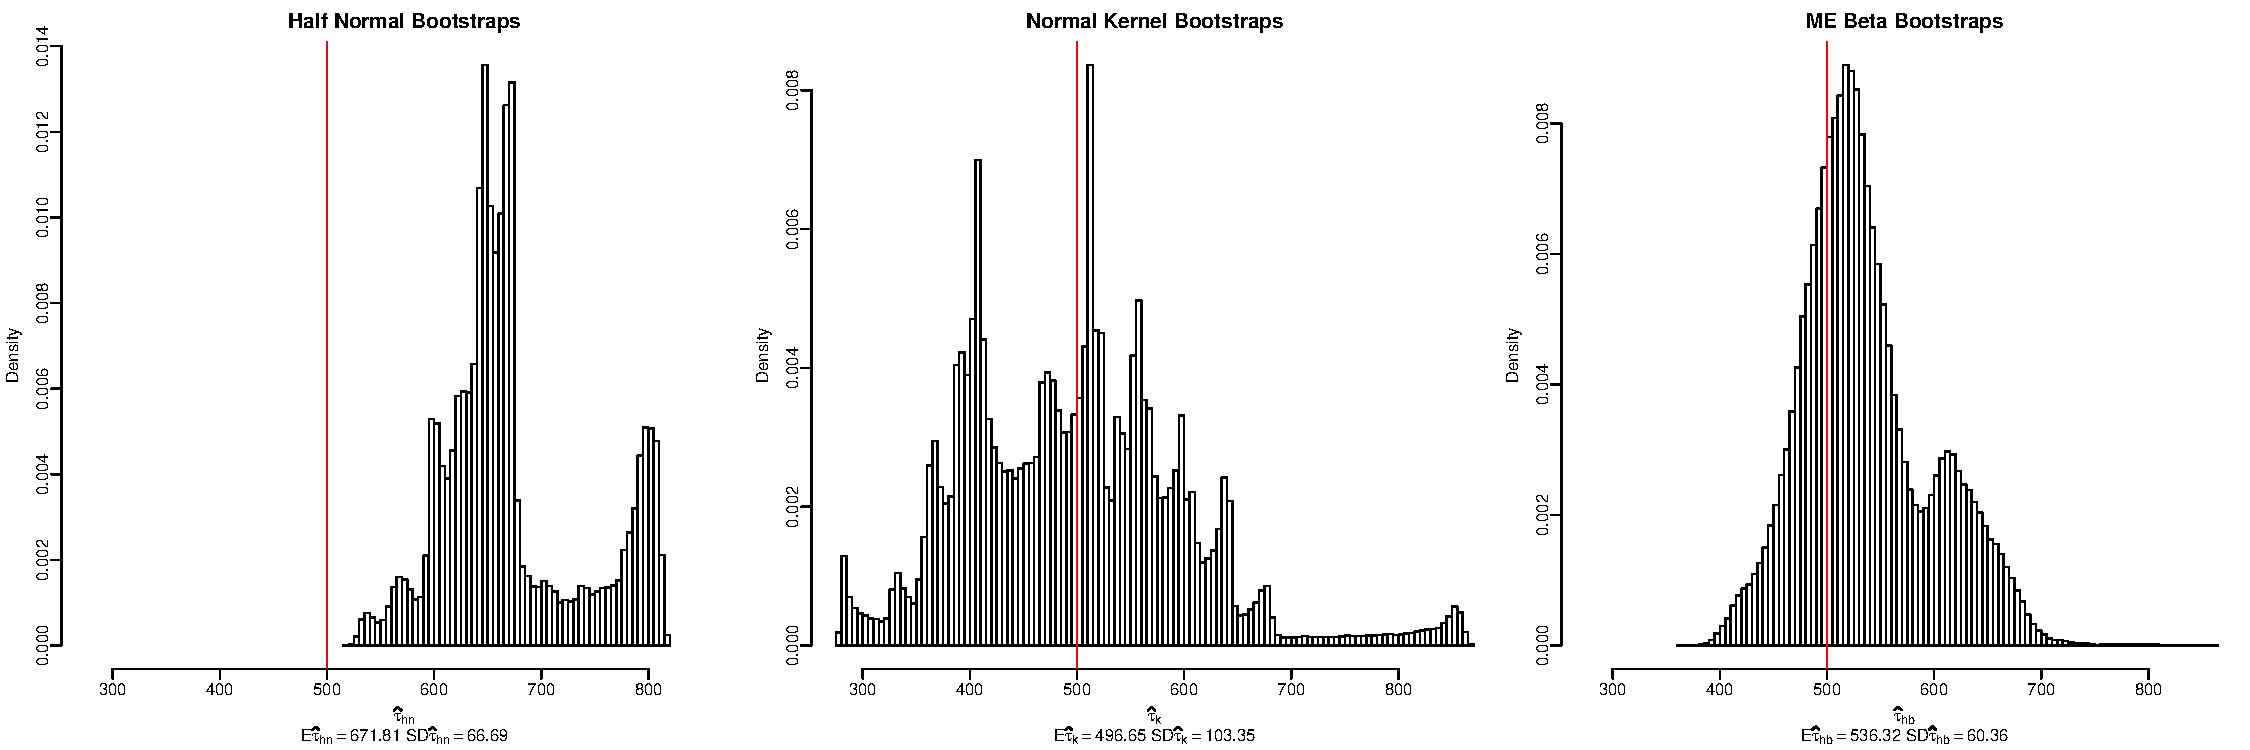
\includegraphics[width=\textwidth]{../500K_bootstrap_comparison.pdf}
  We estimated the total $\tau = 500$ with 500,000 ideal bootstrap systematic samples using half-normal estimation, normal kernel estimation with the recommended kernel width \cite{thompson2012sampling}, 
  and EM half-beta estimation with histogram bin sizes given by the Sturges method.
}

%----------------------------------------------------------------------------------------
%	Entropy Maximizing Algorithm
%----------------------------------------------------------------------------------------

\headerbox{Density Estimation with Entropy Maximization}{name=method1,column=0,span=2,below=introduction}{ % This block's bottom aligns with the bottom of the results block

\begin{multicols}{2}
  The beta parametric family provides a flexible collection of functions that
  have sufficiently low kurtosis to fit the problematic distance data given in
  the introduction. If we reflect the distance data about zero and rescale to
  $[0,1]$, we can fit the data to a half-beta distribution by optimizing our
  entropy estimate. This leads to the following optimization problem for
  estimating a symmetric density supported on a finite interval:
  \begin{equation}
    \hat f = \argmin_{f \in \mathrm{beta}} \widehat H (f)^{-1}
  \end{equation}
  To mimic Anderson and Pospahala's data, we conducted a simulation where detected points were given by Bernouli trials with probabilities 
  \begin{equation}
    p(d) = 
    \begin{cases}
      1 & |d| < e\\
      (1-d)^p & |d| < b\, e.
    \end{cases}
  \end{equation}
  
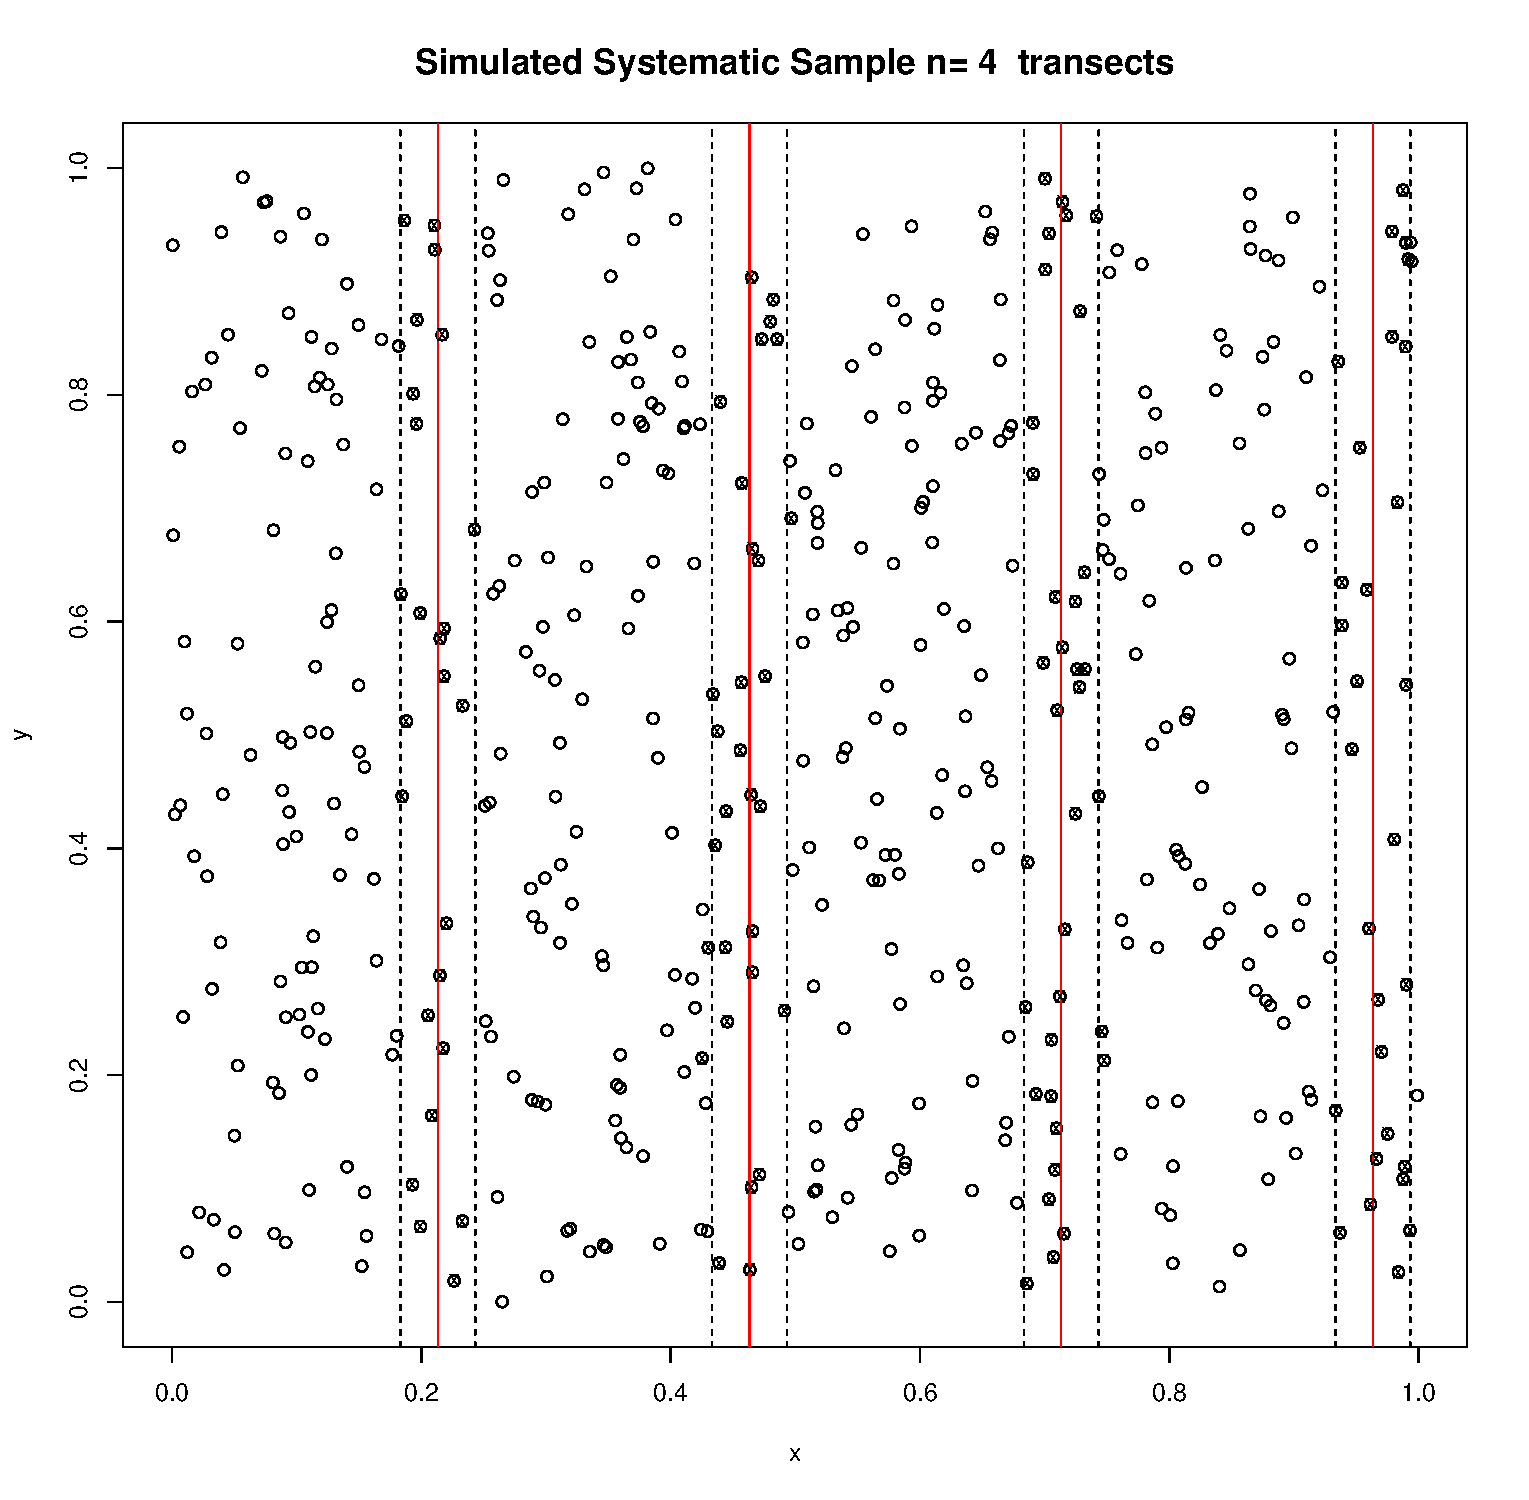
\includegraphics[width=.45\textwidth]{../simulated_sample.pdf}
\end{multicols}
}

\end{poster}

\end{document}
